%-------------------------------------------------------------------------------
% File: architecture.tex
%
% Author: Marco Pinna
%         Created on <date>
%-------------------------------------------------------------------------------
\chapter{Architecture}\label{ch:architecture}

As mentioned in \ref{sec:possible_architectures}, two architectures were identified to implement the algorithm: the first one carries out the procedure in a \textbf{bitwise} fashion; the second one works \textbf{bytewise} by means of a look-up table (LUT).\\
In this chapter both the architectures will be analysed in detail, showing advantages and drawbacks of the two.\\
The initial stage of the development process followed a top-down approach to identify the individual components that would comprise the entire architecture. For each component, it was studied which simpler sub-components it should consist of.\\
The whole development process of the components was carried out with modularity in mind, so as to ease the reuse of them in the different architectures.\\

\section{Bitwise architecture}\label{sec:bitwise_arch}

Figure \ref{fig:block_diagram_bitwise} shows a high-level view of the bitwise architecture of the CRC (clocks and resets are not shown for the sake of clarity).\\
The architecture is divided in \textbf{datapath} (black connections) and \textbf{control unit} (red connections). The datapath consists of all the register, and processing or combinatorial units required to execute each step of the algorithm. The control unit takes care of issuing, at certain clock cycles, specific control signals to the datapath, to ensure the correct execution of each step of the algorithm.\\
\hfill \break
Light grey rectangles are \textbf{registers} made of D Flip-Flops;\\
dark grey rectangles are a different kind of registers whose basic unit is a \textit{Double Data Flip-Flop (D2FF)}, whose architecture will be discussed later; this allows to build a register with two different inputs (e.g. the accumulator) or a Parallel-Input-Parallel-Output (\textit{PIPO}) Shift Register;\\
the light blue block is a purely combinatorial block which implements a XOR between the input and the CRC generator polynomial G (the most significant bit of the input behaves as a sort of \textit{enable}, i.e. when it is \texttt{0} the combinatorial block will act as if it was transparent).\\

\begin{figure}[H]
    \begin{center}
        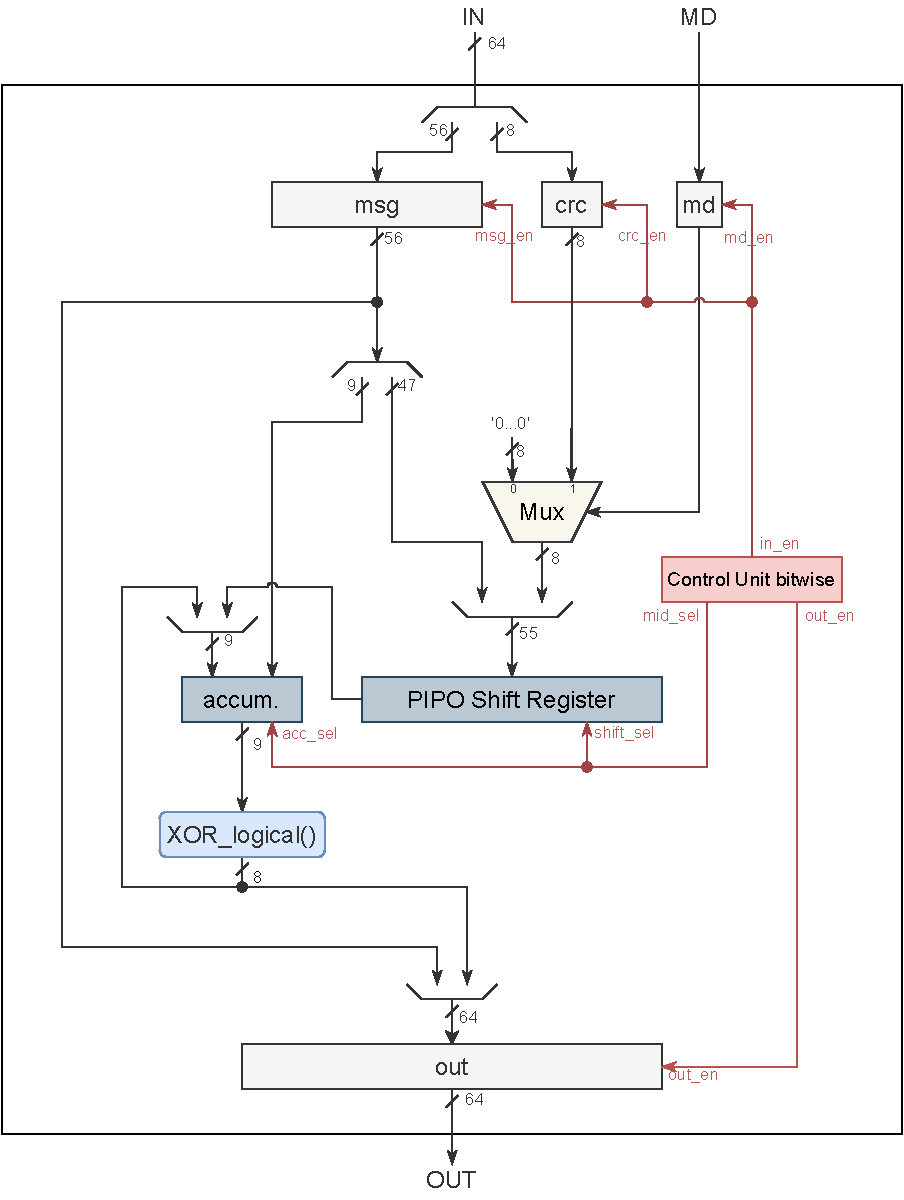
\includegraphics[scale=.85,clip]{img/block_diagram_bitwise.pdf}
    \end{center}
    \vspace*{-0.5cm}
    \caption{Block diagram of the bitwise implementation of the CRC.}
    \label{fig:block_diagram_bitwise}
\end{figure}

\hfill \break
The bitwise CRC works as follows:
\begin{itemize}
	\item Input data is read from \texttt{IN} and \texttt{MD} and stored into the input registers \texttt{msg}, \texttt{crc} and \texttt{md}
	\item Input data is then fed into the processing section of the circuit, which computes the polynomial long division advancing bit by bit.
	\item At the end of the computation, the original message along with the CRC (or the CRC check, depending on the input value of \texttt{MD}) is placed into the output register \texttt{out}.
\end{itemize}

The following pseudocode shows what happens during each clock cycle, in a finite-state machine fashion:
\hfill \break

\lstset{style=codestyle}\label{code:FSM_bitwise}
\lstinputlisting[language=python,caption={FSM pseudocode of bitwise architecture}]{code/FSM_bitwise.py}
\hfill \break
A total of 5 different phases can be identified. This is reflected in the internal logic of the relative Control Unit\\

\section{LUT-based architecture}\label{sec:LUT_arch}


Figure \ref{fig:block_diagram_lut} shows a high-level view of the LUT-based architecture of the CRC (clocks and resets are not shown for the sake of clarity).\\
As it can be seen, the structure is quite similar to the bitwise one: it only differs by some minor changes in the sizes of signals and registers and in the feedback loop that goes back into the accumulator.\\
The light blue block is a combinatorial network that contains a pre-computed 1x256B look-up table.\\
\hfill \break
The LUT-based CRC works as follows:\\
\begin{itemize}
	\item Input data is read from \texttt{IN} and \texttt{MD} and stored into the input registers \texttt{msg}, \texttt{crc} and \texttt{md}
	\item Input data is then fed into the processing section of the circuit, which computes the polynomial long division advancing byte by byte.
	\item At the end of the computation, the original message along with the CRC (or the CRC check, depending on the input value of \texttt{MD}) is placed into the output register \texttt{out}.
\end{itemize}

\begin{figure}[H]
    \begin{center}
        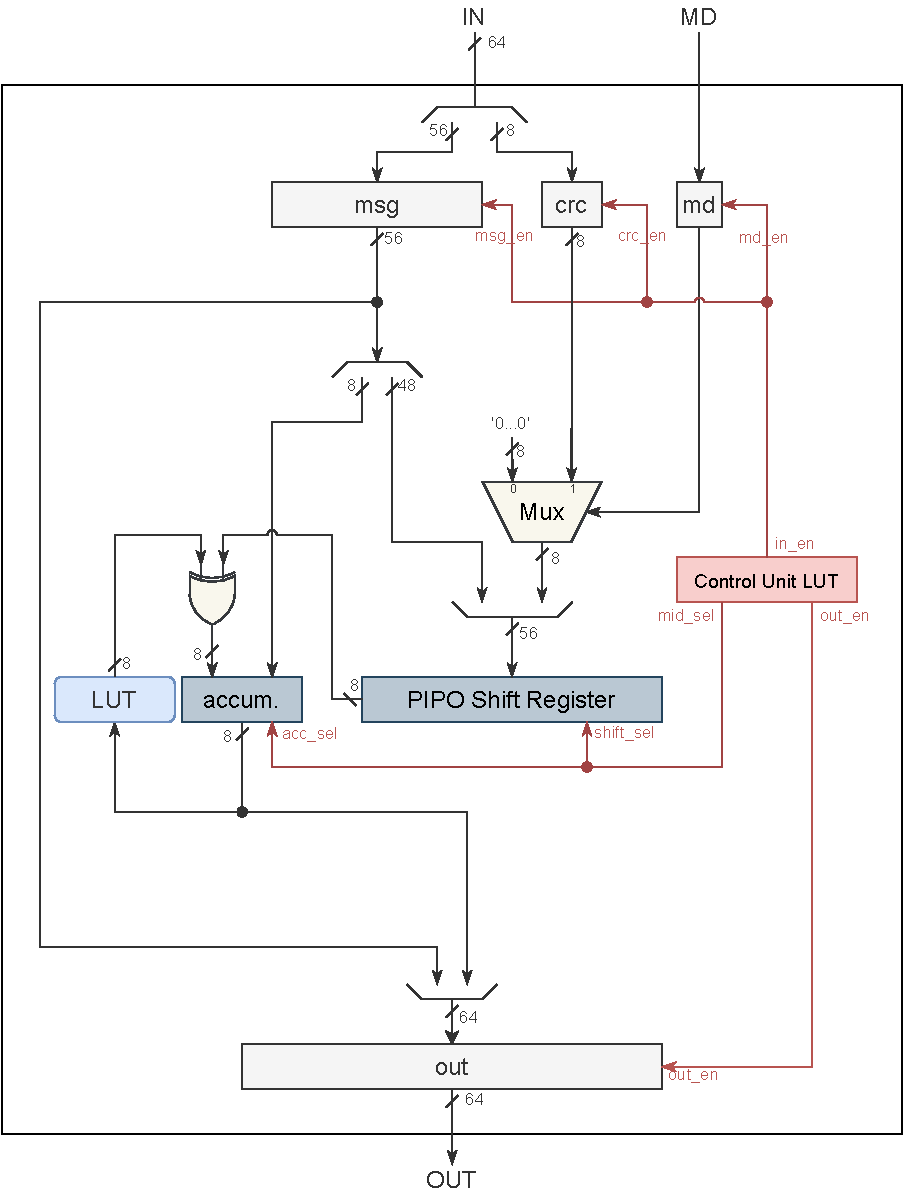
\includegraphics[scale=.85,clip]{img/block_diagram_lut.pdf}
    \end{center}
    \vspace*{-0.5cm}
    \caption{Block diagram of the LUT-based implementation of the CRC.}
    \label{fig:block_diagram_lut}
\end{figure}

\
The following pseudocode shows what happens during each clock cycle, in a finite-state machine fashion:
\pagebreak

\lstset{style=codestyle}\label{code:FSM_LUT}
\lstinputlisting[language=python,label=code:FSM_LUT,caption={FSM pseudocode of LUT based architecture}]{code/FSM_LUT.py}
\hfill \break
Analogously to the previous architecture, a total of 5 different phases can be identified in this one too.\\
\hfill \break
As it can be seen by the clock numbers, the actual computation phases in this architecture are only 7 clock cycles long, against 55 clock cycles of the former architecture. Both architecture further have 2 preliminary clock cycles to read the inputs and 1 final clock cycle to set the output. This yields a total of 58 and 10 clock cycles respectively.\\
The speed-up factor obtained from the second implementation is therefore equal to 5.8, provided the clock frequency is equal. This clock frequency assumption will be tested in chapter \ref{ch:synth_results} during the synthesis process.

\section{Subcomponents}\label{sec:subcomponents}
In this section the various subcomponents that make up the two architectures will be analyzed.

\subsection{Double Data Flip Flop (D2FF)}\label{subsec:d2ff}

\begin{figure}[H]
    \begin{center}
        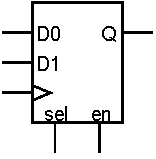
\includegraphics[scale=1.3,clip]{img/DFF_block.pdf}
    \end{center}
    \vspace*{-0.5cm}
    \caption{D2FF.}
    \label{fig:DFF_block}
\end{figure}

The \textbf{D2FF (Double Data Flip Flop)} is the basic unit the accumulator and the shift register are made of.\\
It is similar to a common D Flip-Flop, with the only difference that it has two different data inputs (hence the name), \texttt{d0} and \texttt{d1}, and a \texttt{sel} input which controls which of the two data inputs goes to the output \texttt{q}.\\
Its truth table is the following:\\

\begin{table}[H]
\centering
\begin{tabular}{|c|c|c|c|c|c|}
\hline
\texttt{clk}            & \texttt{en}        & \texttt{sel}       & \texttt{D0}        & \texttt{D1}        & \texttt{Q\textsubscript{next}} \\ \hline
non-rising              & X                  & X                  & X                  & X                  & Q                    \\ \hline
\multirow{5}{*}{rising} & 0                  & X                  & X                  & X                  & Q                    \\ \cline{2-6} 
                        & \multirow{4}{*}{1} & \multirow{2}{*}{0} & 0                  & \multirow{2}{*}{X} & 0                    \\ \cline{4-4} \cline{6-6} 
                        &                    &                    & 1                  &                    & 1                    \\ \cline{3-6} 
                        &                    & \multirow{2}{*}{1} & \multirow{2}{*}{X} & 0                  & 0                    \\ \cline{5-6} 
                        &                    &                    &                    & 1                  & 1                    \\ \hline
\end{tabular}
\end{table}

\subsection{D2FF-N}\label{subsec:d2ffn}

\begin{figure}[H]
    \begin{center}
        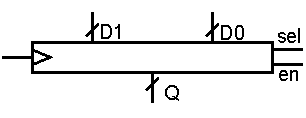
\includegraphics[scale=1.1,clip]{img/DFF_N_block.pdf}
    \end{center}
    \vspace*{-0.5cm}
    \caption{D2FF-N.}
    \label{fig:DFFNblock}
\end{figure}

The accumulator is an instance of a \textbf{D2FF-N}, i.e. a register of N bits with 2 N-bit data inputs and a \texttt{sel} input to toggle between them.\\
Just as classical registers are arrays of D Flip Flops, a D2FF-N is an array of D2FF: its \texttt{en}, \texttt{sel} and \texttt{clk} are mapped to the respective input of each individual D2FF and the i-th bit of the inputs and the output is mapped accordingly to the respective input or output of the i-th D2FF.

\subsection{PIPO Shift Register}\label{subsec:PIPOshiftreg}

\begin{figure}[H]
    \begin{center}
        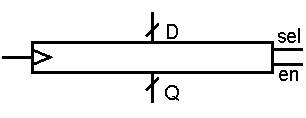
\includegraphics[scale=1.1,clip]{img/PIPO_shiftreg_block.pdf}
    \end{center}
    \vspace*{-0.5cm}
    \caption{PIPO Shift Register.}
    \label{fig:PIPOshiftregblock}
\end{figure}
The \textbf{PIPO (Parallel-Input-Parallel-Output) Shift Register} is a shift register whose input and output can be written/read in parallel. It is also an array of D2FF, but the \texttt{d1} input of each D2FF is connected to the \texttt{q} output of the previous one (except for the very first D2FF which always reads \texttt{0}). The \texttt{sel} input therefore acts as a \textit{switch} which can enable/disable the shifting.

\subsection{Control Unit}\label{subsec:CU}
\begin{figure}[H]
    \begin{center}
        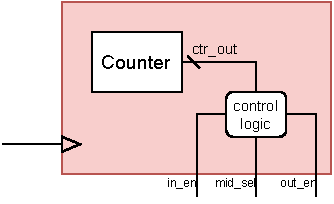
\includegraphics[scale=1.3,clip]{img/CU_block.pdf}
    \end{center}
    \vspace*{-0.5cm}
    \caption{Control Unit.}
    \label{fig:CUblock}
\end{figure}

The \textbf{Control Unit} is made of a counter plus some simple control logic that, depending on the output of the counter, issues the correct commands via the  output signals \texttt{in\_en}, \texttt{mid\_sel} and \texttt{out\_en}, the three of which are connected respectively to the input registers \textit{enable}, the accumulator and shift register \textit{select} and the output register \textit{enable}.\\
Depending on the architecture, the control unit will differ in the maximum count and the control logic (cfr. pseudocode in Listings \ref{code:FSM_bitwise} and \ref{code:FSM_LUT}).\\
\hfill \break
\hfill \break
Both architectures were designed with the following assumption in mind:\\
the upstream and downstream circuits (with respect to the CRC circuit) are both synchronous with the designed component and they know how many clock every implementation takes to compute the CRC.\\
Should this assumption fall, a handshake mechanism would be required, both for the producer (upstream) component and for the consumer (downstream) component.\\
The \textit{phases-structured} logic lends itself well to this type of addition: the two handshakes would be connected to the Control Unit, which could pause/resume the advance of the counter and keep the circuit in the first (last) phase as long as it is required for the producer or consumer to write or read the data.